\subsection{Other meshes}
In this section, some other mesh examples with irregular geometric boundaries are considered.
Fig.~\ref{}
\begin{figure}[h!]
    \begin{subfigure}[b]{1\linewidth}
        \centering
        \scalebox{0.3}{
            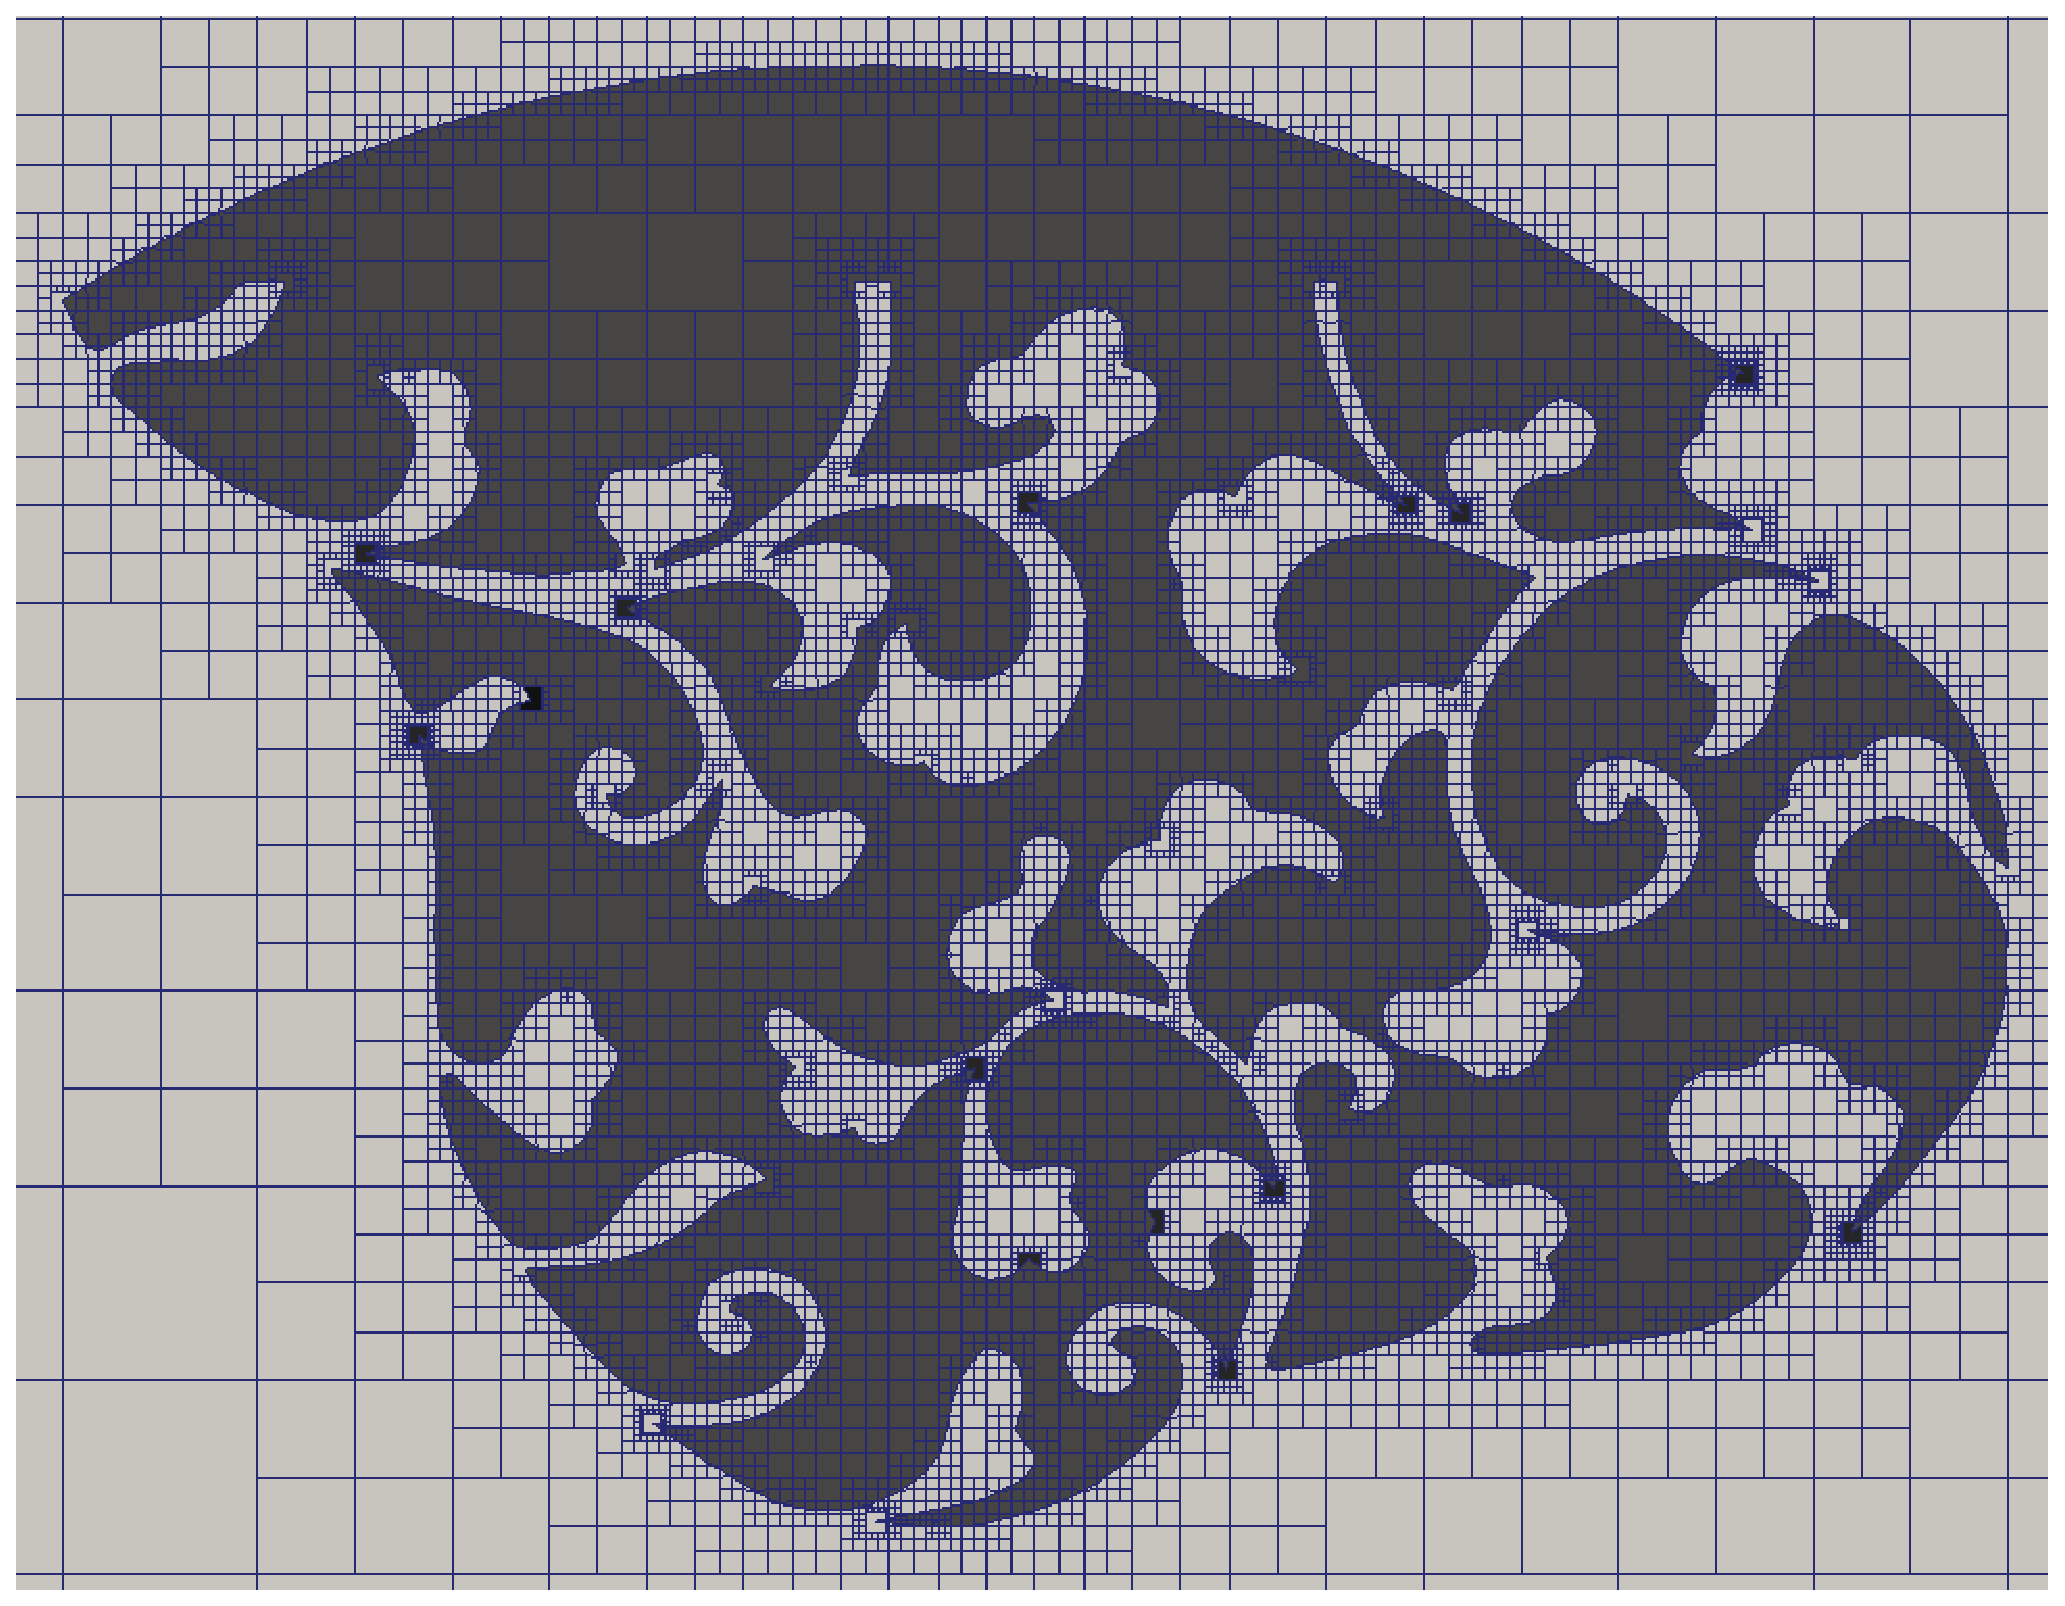
\includegraphics{quadtree/ex_images/qdt_ex_mesh_flower.eps}
        }
        \caption{Mesh for flowers}
    \end{subfigure}
    \\
    \begin{subfigure}[b]{1\linewidth}
        \centering
        \scalebox{0.3}{
            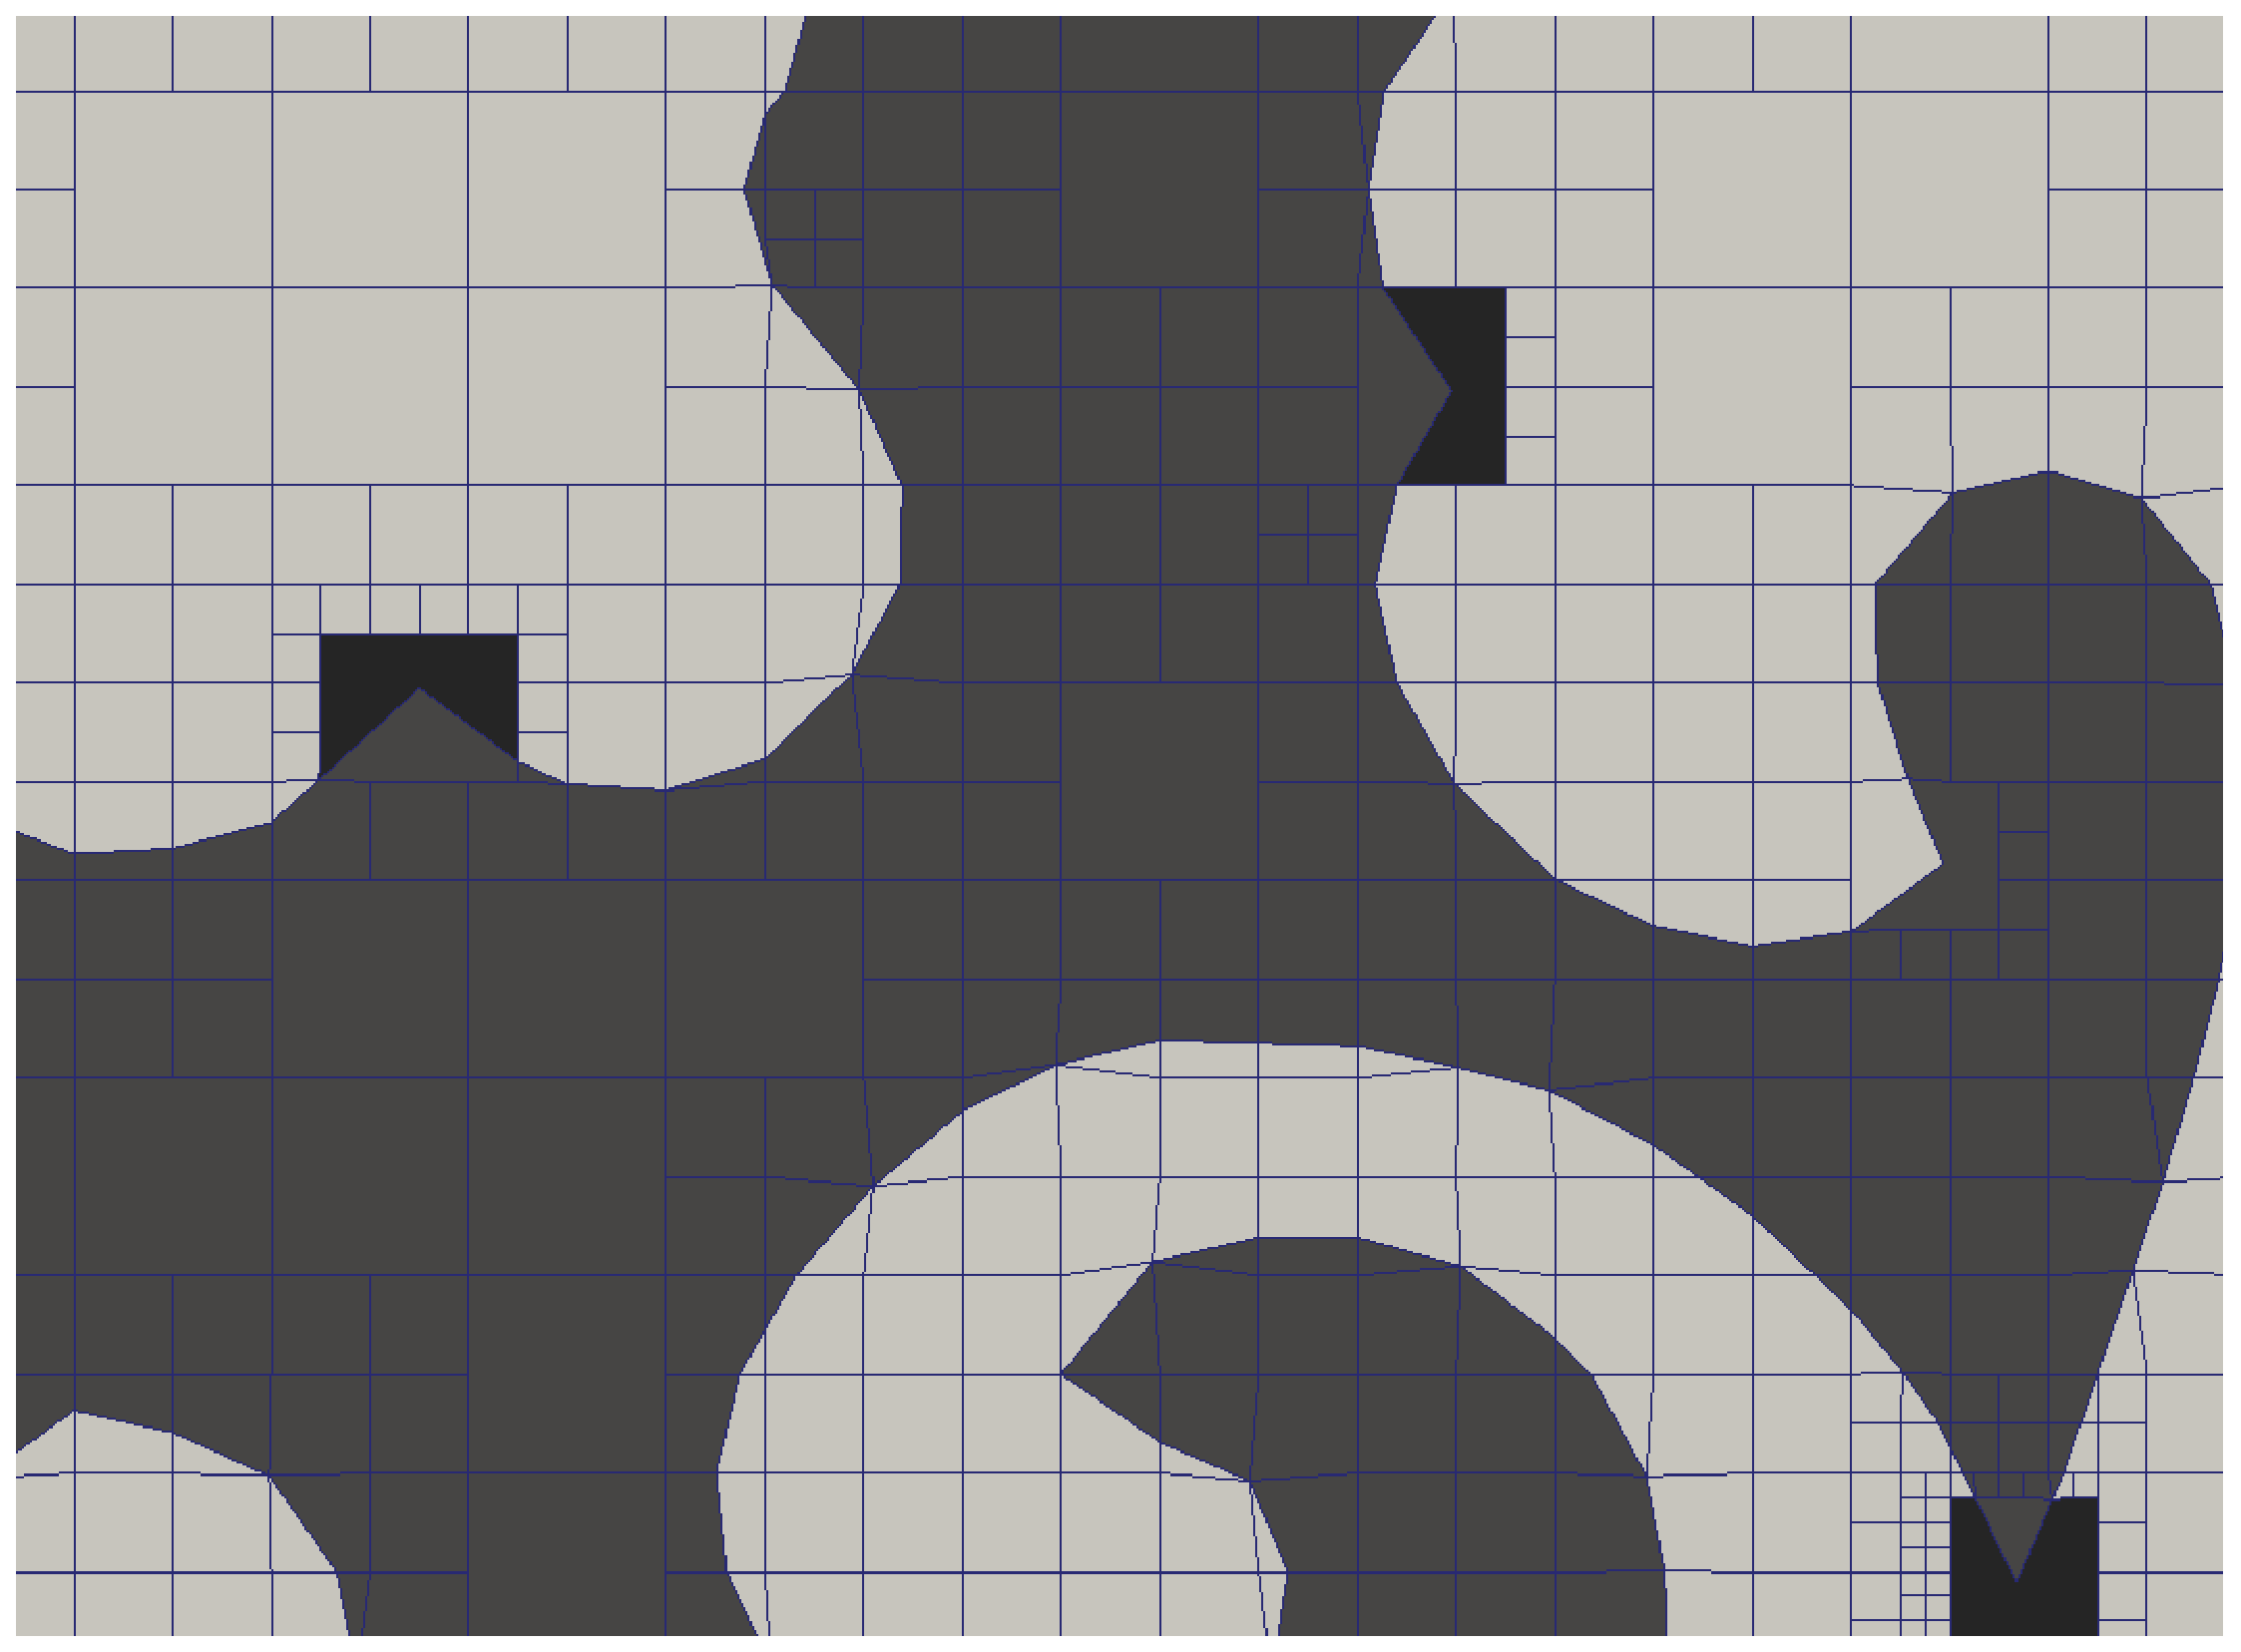
\includegraphics{quadtree/ex_images/qdt_ex_mesh_flower_sharp_corners.eps}
        }
        \caption{Mesh for flowers : Sharp corners treatment}
    \end{subfigure}

\end{figure}

\begin{figure}[h!]
    \begin{subfigure}[b]{1\linewidth}
        \centering
        \scalebox{0.3}{
            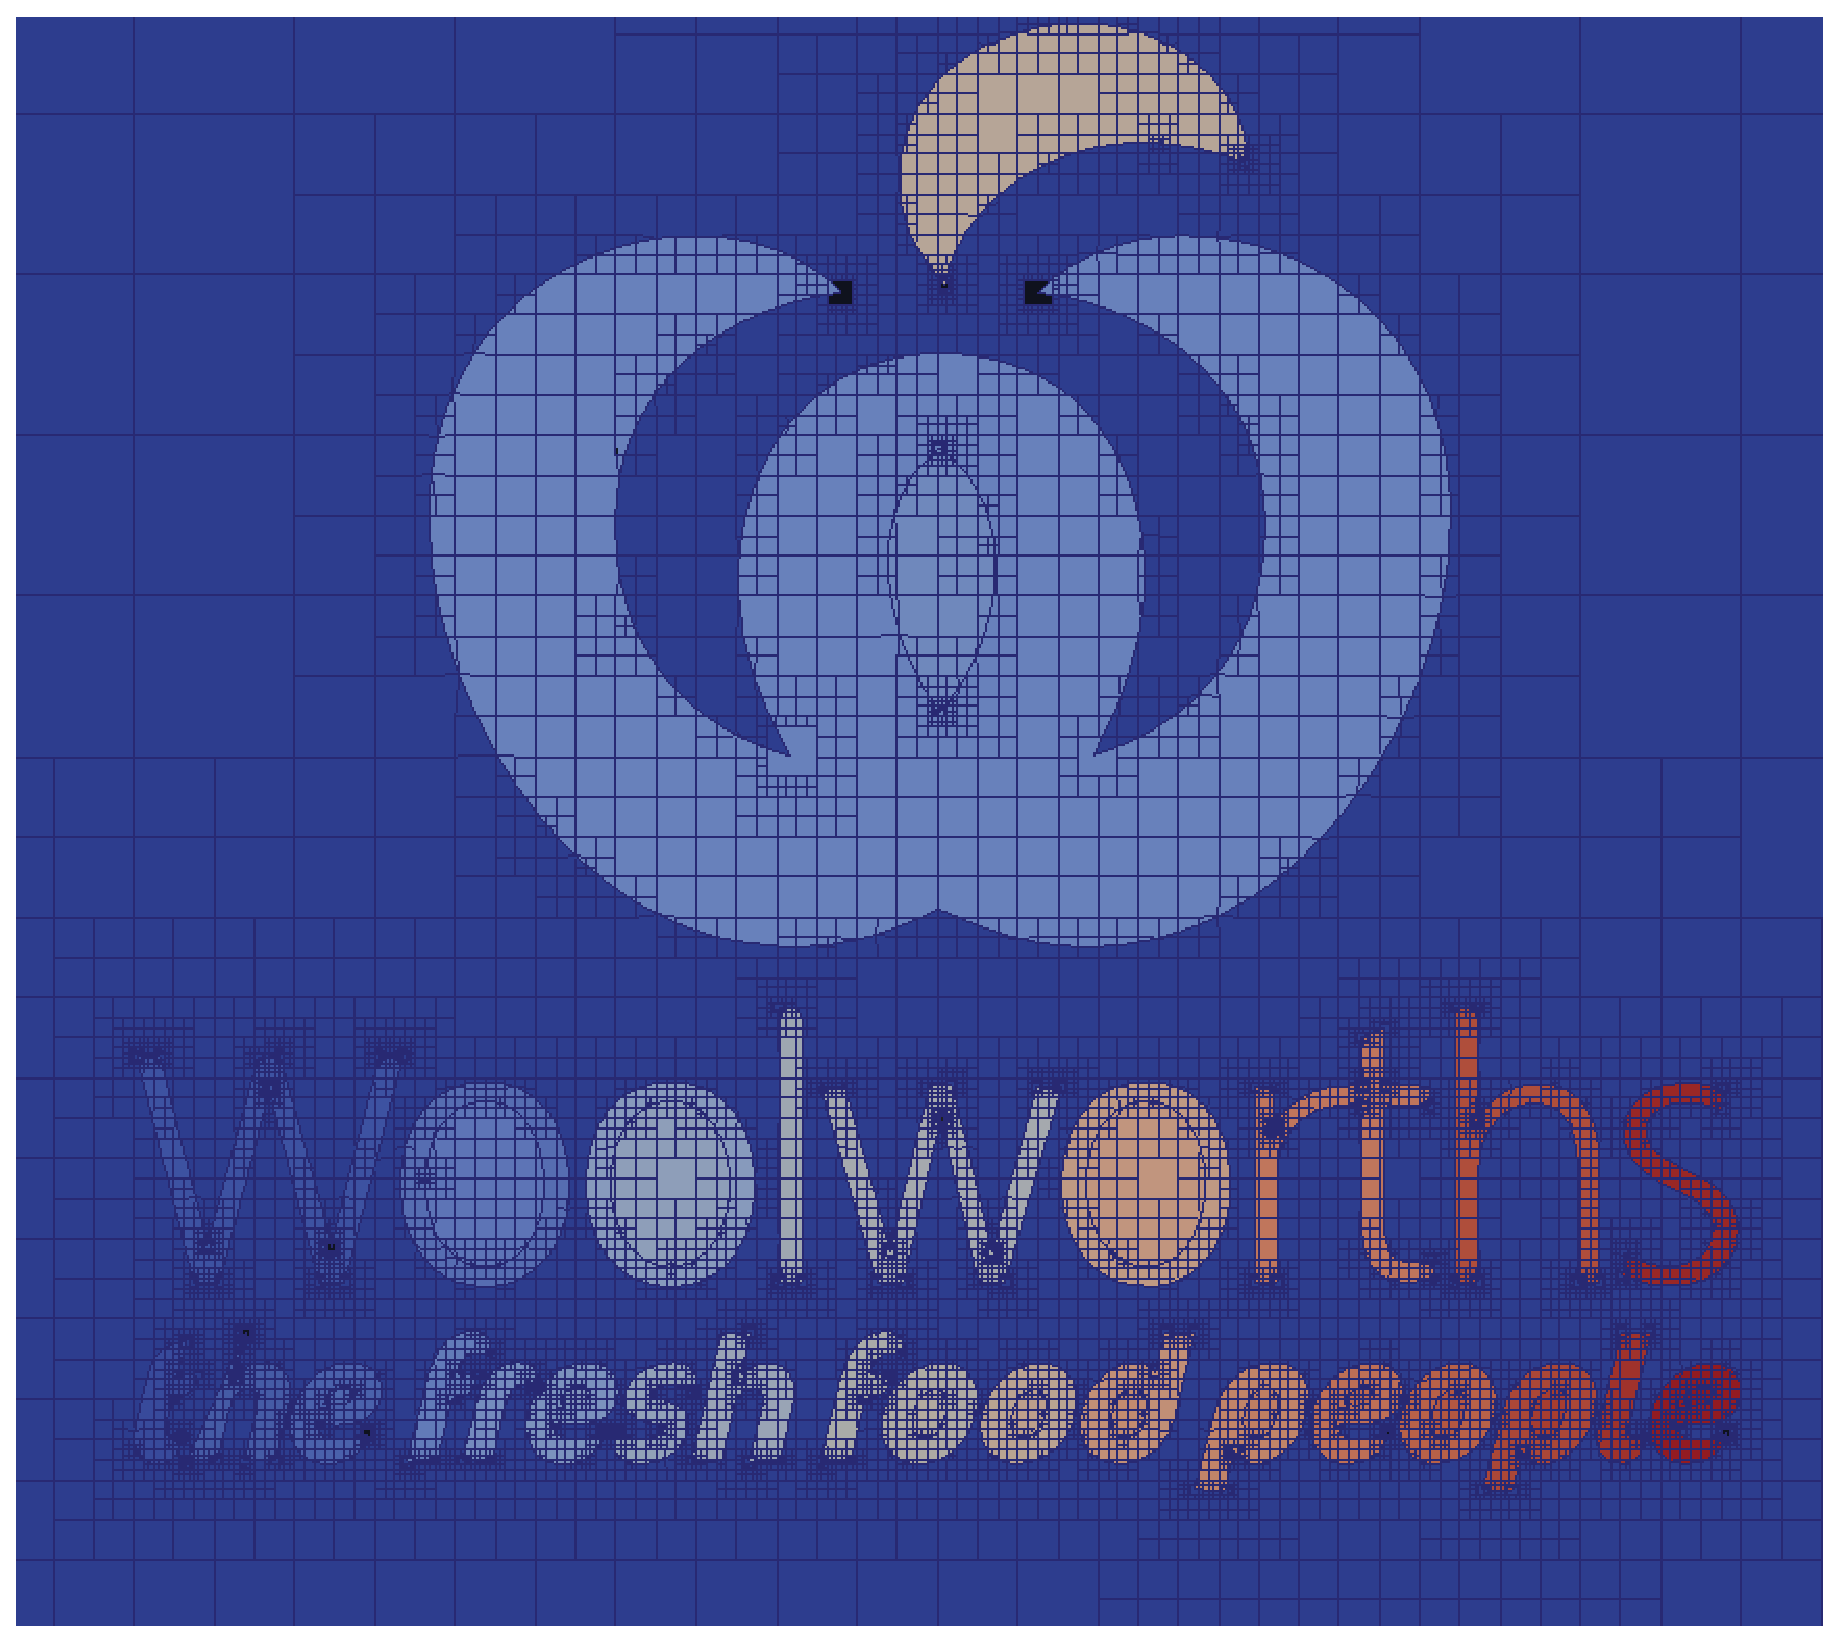
\includegraphics{quadtree/ex_images/qdt_ex_mesh_wolli.eps}
        }
        \caption{Mesh for woolworth logo : Different colors for differnet materials}
    \end{subfigure}
    \\
    \begin{subfigure}[b]{1\linewidth}
        \centering
        \scalebox{0.3}{
            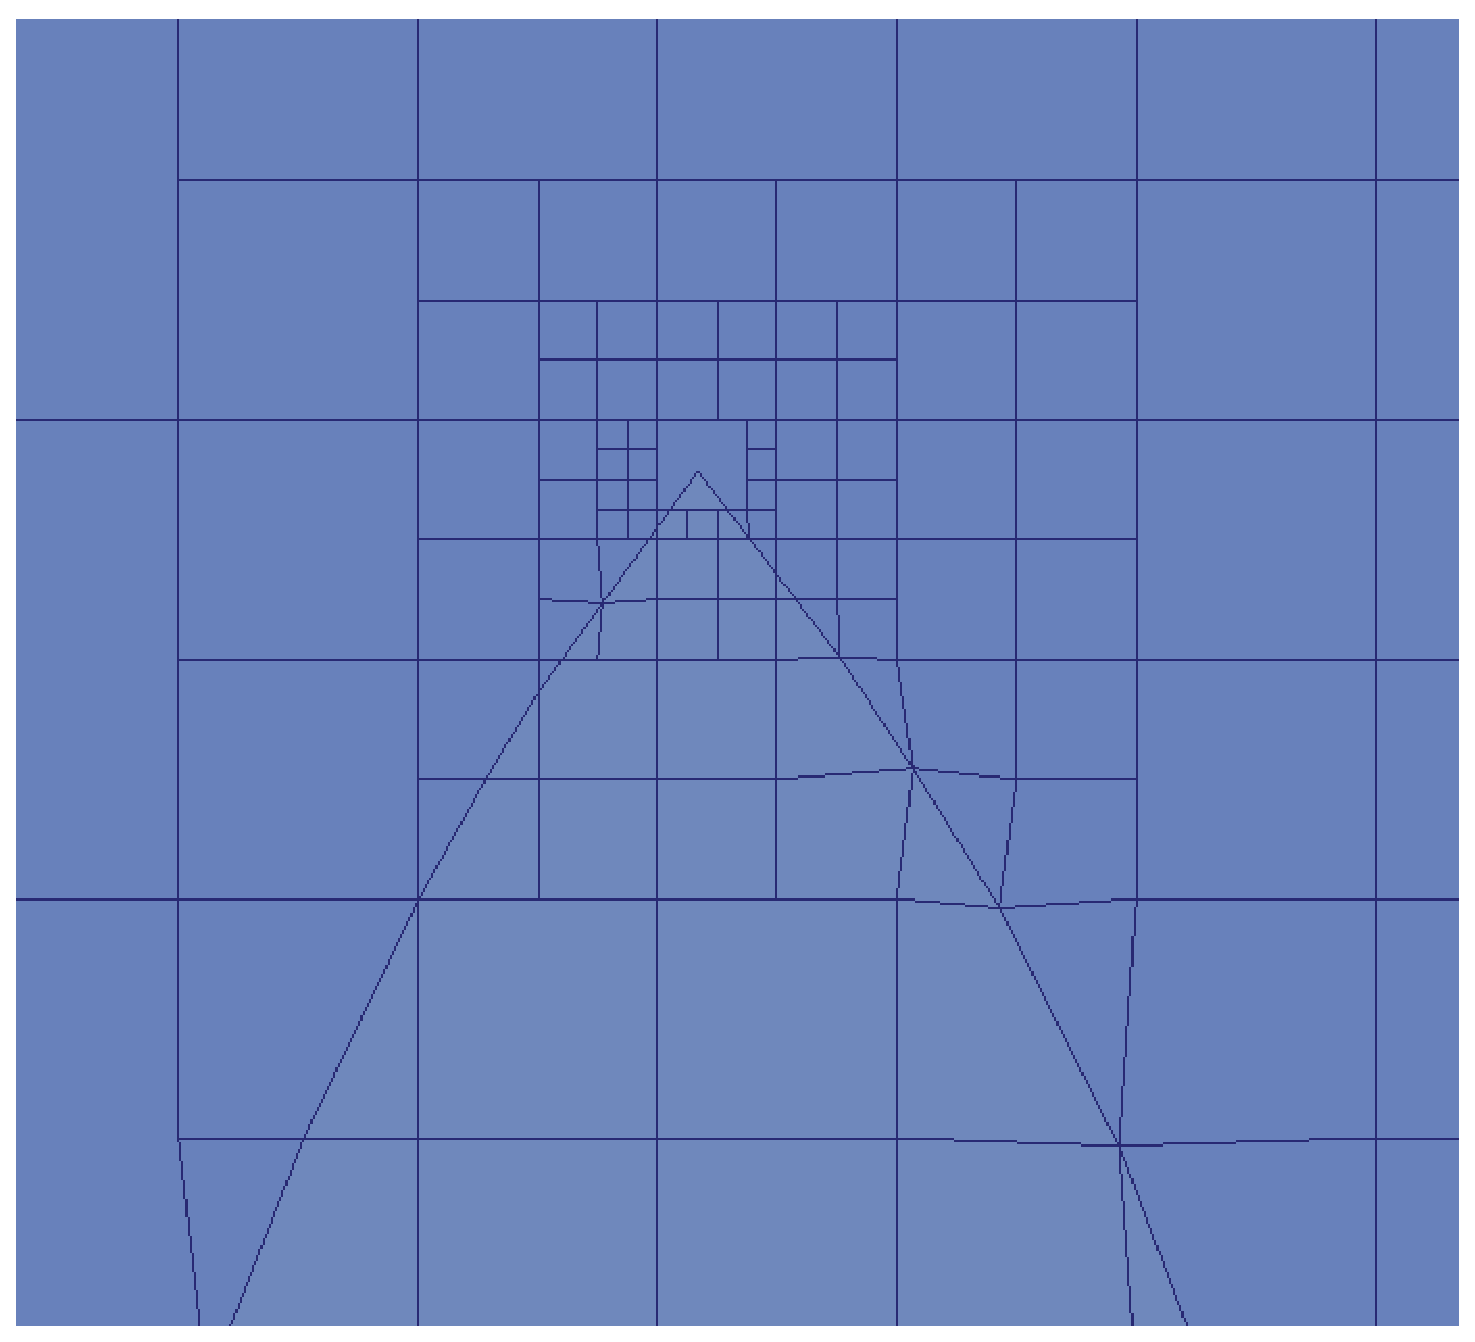
\includegraphics{quadtree/ex_images/qdt_ex_mesh_wolli_sharp_corner.eps}
        }
        \caption{Mesh for woolworth logo : Sharp conors treatment}
    \end{subfigure}
\end{figure}
